% chinthakawk@gmail.com

\documentclass[compress]{beamer} %this is to use copressed header from the
\usepackage{etex}
\usepackage{beamerthemeshadow} %our theme, later you can change it
\usepackage[frenchb]{babel}
\usepackage{fancyhdr} % Required for custom headers
\usepackage[utf8]{inputenc}
\usepackage[lined,boxed]{algorithm2e}
\usepackage[all]{xy}
\usepackage{animate} %need the animate.sty file
\graphicspath{{./Figure/}} 
% editing header
\setbeamertemplate{headline}
{
  \leavevmode%
  \hbox{%
  \begin{beamercolorbox}[wd=.5\paperwidth,ht=2.25ex,dp=1.8ex,leftskip=1em,left]{section in head/foot}%
    \usebeamerfont{subsection in head/foot}\hspace*{5ex}\insertsectionhead
  \end{beamercolorbox}%
  \begin{beamercolorbox}[wd=.5\paperwidth,ht=2.25ex,dp=1.8ex,left,leftskip=1em]{subsection in head/foot}%
    \usebeamerfont{section in head/foot}\insertshorttitle\hspace*{2ex}
  \end{beamercolorbox}}%
  \vskip0pt%
}

% editing footer
\setbeamertemplate{footline}
{
  \leavevmode%
  \hbox{%
  \begin{beamercolorbox}[wd=.5\paperwidth,ht=2.25ex,dp=1ex,right]{author in head/foot}%
    \usebeamerfont{author in head/foot}\insertshortauthor\hspace*{2ex}
  \end{beamercolorbox}%
  \begin{beamercolorbox}[wd=.5\paperwidth,ht=2.25ex,dp=1ex,right]{date in head/foot}%
    \usebeamerfont{date in head/foot}\insertshortdate{}\hspace*{2em}
    \insertframenumber{} / \inserttotalframenumber\hspace*{2ex} 
  \end{beamercolorbox}}%
  \vskip0pt%
}
\definecolor{orange}{rgb}{1,0.5,0}
\definecolor{darkgreen}{rgb}{0,0.5,0}
\definecolor{darkblue}{rgb}{0,0,0.5}

\def\etal{et al.\ }
\def\ie{i.e.\ }
\def\eg{e.g.\ }

%put a wide hat over the argumetn
\newcommand{\lift}[1]{\ensuremath{\widehat{#1}}}

%put a wide hat over the argumetn
%\newcommand{\lifto}[1]{\ensuremath{\check{#1}}}
\newcommand{\lifto}[1]{\ensuremath{\overset{_{_{\circ}}}{#1}}}


% stack vector
\newcommand{\stackv}[1]{\ensuremath{\vet{v}\left( {#1} \right)}}
\newcommand{\ustackv}[1]{\ensuremath{\inv{\vet{v}}\left( {#1} \right)}}

% symmetric stack vector
\newcommand{\stackvs}[1]{\ensuremath{\vet{v}_{\textit{sym}}\left( {#1} \right)}}

% Matrix Lifting: put a wide hat over the argument intended to be a matrix
\newcommand{\mlift}[1]{\ensuremath{\lift{\mat{#1}}}}
\newcommand{\mlifto}[1]{\ensuremath{\lifto{\mat{#1}}}}

% Vector Lifting: put a wide hat over the argument intended to be a matrix
\newcommand{\vlift}[1]{\ensuremath{\lift{\vet{#1}}}}
\newcommand{\vlifto}[1]{\ensuremath{\lifto{\vet{#1}}}}

\newcommand{\bmat}[1]{\ensuremath{\begin{bmatrix} #1 \end{bmatrix}}}
% Vector: print the argument as a vector
\newcommand{\vet}[1]{\ensuremath{\mathbf{#1}}}

% Matrix: print the argument as a matrix
\newcommand{\mat}[1]{\ensuremath{\,\mathtt{#1}\,}}

% Inverse: print a -1 on the top right of the argument 
\newcommand{\inv}[1]{\ensuremath{{#1}^{\text{-}1}}}

% Inverse: print a -1 on the top right of the argument 
\newcommand{\minv}[1]{\ensuremath{\mat{{#1}}^{\text{-}1}}}

% Transpose: print a T on the top right of the argument 
\newcommand{\tra}[1]{\ensuremath{{#1}^{\!\mathsf{T}}}}

% Transpose Matrix: print a T on the top right of the argument intended to be a matrix 
\newcommand{\mtra}[1]{\ensuremath{\tra{\mat{#1}}}}

% Transpose Vector: print a T on the top right of the argument intended to be a vector
\newcommand{\vtra}[1]{\ensuremath{\tra{\vet{#1}}}}

% minus transpose:  print a -T on the top right of the argument
\newcommand{\ment}[1]{\ensuremath{{#1}^{\text{-}\mathsf{T}}}}

% minus transpose matrix:  print a -T on the top right of the argument
\newcommand{\mment}[1]{\ensuremath{{\mat{#1}}^{\text{-}\mathsf{T}}}}

% Cross Matrix:  print the argument in the cross matrix notation
\newcommand{\crmat}[1]{\ensuremath{\left[{#1}\right]_{\times}}}

%random variable
\newcommand{\rand}[1]{\ensuremath{\mathbb{#1}}}

%insert 2 figures on a row
\newcommand{\insertTwoF}[4]{
  \begin{figure}[h!]
    \centering
    \begin{minipage}{#4\linewidth}
    \includegraphics[width=\linewidth]{#1}
    \end{minipage}
    \begin{minipage}{#4\linewidth}
    \includegraphics[width=\linewidth]{#2}
    \end{minipage}
      \caption{#3}
  \end{figure}  
}

\newcommand{\insertF}[3]{
  \begin{figure}[h!]
    \centering
    \begin{minipage}{#3\linewidth}
    \includegraphics[width=\linewidth]{#1}
    \end{minipage}  
      \caption{#2}
  \end{figure}  
}

%enable numbering captions for the images
\setbeamertemplate{caption}[numbered]



%begining of the doc
\begin{document}

 \title{Statistic Criterion for Patch Comparison}  
 %\author{Jia LI}
 %\date{August, 2013} 

 %title page
 \begin{frame}
\titlepage
    \centering
    \begin{minipage}{0.4\textwidth}
    \begin{flushleft} \large
    \emph{Author:}\\
    Dalens Théophile\\
    LI Jia\\
    
    \end{flushleft}
    \end{minipage}
    \begin{minipage}{0.4\textwidth}
    \begin{flushright} \large
    \emph{Course:}\\
    Imagerie Satellitaire
    \end{flushright}
    \end{minipage}\\[3cm]
 \end{frame}
 \section{Introduction}
 \begin{frame}
  \frametitle{Introduction}
  \insertF{ste}{depth map in stereo vision}{0.5}
  \insertF{debruitage}{Non local means denoising}{0.6}
 \end{frame}

 %ToC page
 \begin{frame}
 \scriptsize
 {
 \begin{enumerate}


  \item \textbf{A contrario method}
  \begin{enumerate}
   \item Modeling
   \item Statistic
   \item Approach
   
  \end{enumerate}

  \item Likelihood ratio
  \item Likelihood ratio with learned prior
  \item Comparison
  
 \end{enumerate}

  %\frametitle{Table of contents}
  %\tableofcontents
  
 }
 \end{frame} 
 
 \section{A contrario Method}
 \begin{frame}
  \frametitle{Modeling : principle components analysis}
  \begin{itemize}
     \item A patch is modeled as a random variable $\rand{B}=\rand{C}_i \mat{B}_i$, a linear combination of reference patches, where $\rand{C}_i$ are independent random variable following a distribution $H_i$.
     \item The reference patches are extracted using a PCA algorithm, ($\rand{C}_i$) are supposed to be independent. (uncorrelated indeed)
  \end{itemize}

	\begin{figure}[h!]
	\centering
	\begin{minipage}{0.4\linewidth}
	\includegraphics<1>[width=\linewidth]{zebra.jpg}
	\includegraphics<2>[width=\linewidth]{lena.jpg}
	\includegraphics<3>[width=\linewidth]{wn.png}
	\end{minipage}
	\begin{minipage}{0.4\linewidth}
	\includegraphics<1>[width=\linewidth]{princomp_zebra.png}
	\includegraphics<2>[width=\linewidth]{princomp_lena.png}
	\includegraphics<3>[width=\linewidth]{princomp_wn.png}
	\end{minipage}
	    \caption{Left: a natural image; right: reference patches}
	
	\end{figure}      
 \end{frame}
 
 \begin{frame}
  \frametitle{Modeling : compare with the cosine basis}
We observe that the principle components of a nature image coincide with the cosine basis.
  \begin{figure}[h!]
    \centering
    \begin{minipage}{0.4\linewidth}
    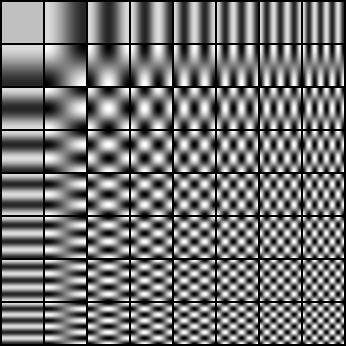
\includegraphics[width=\linewidth]{cosinus_basis.png}
    \end{minipage}
    \begin{minipage}{0.4\linewidth}
    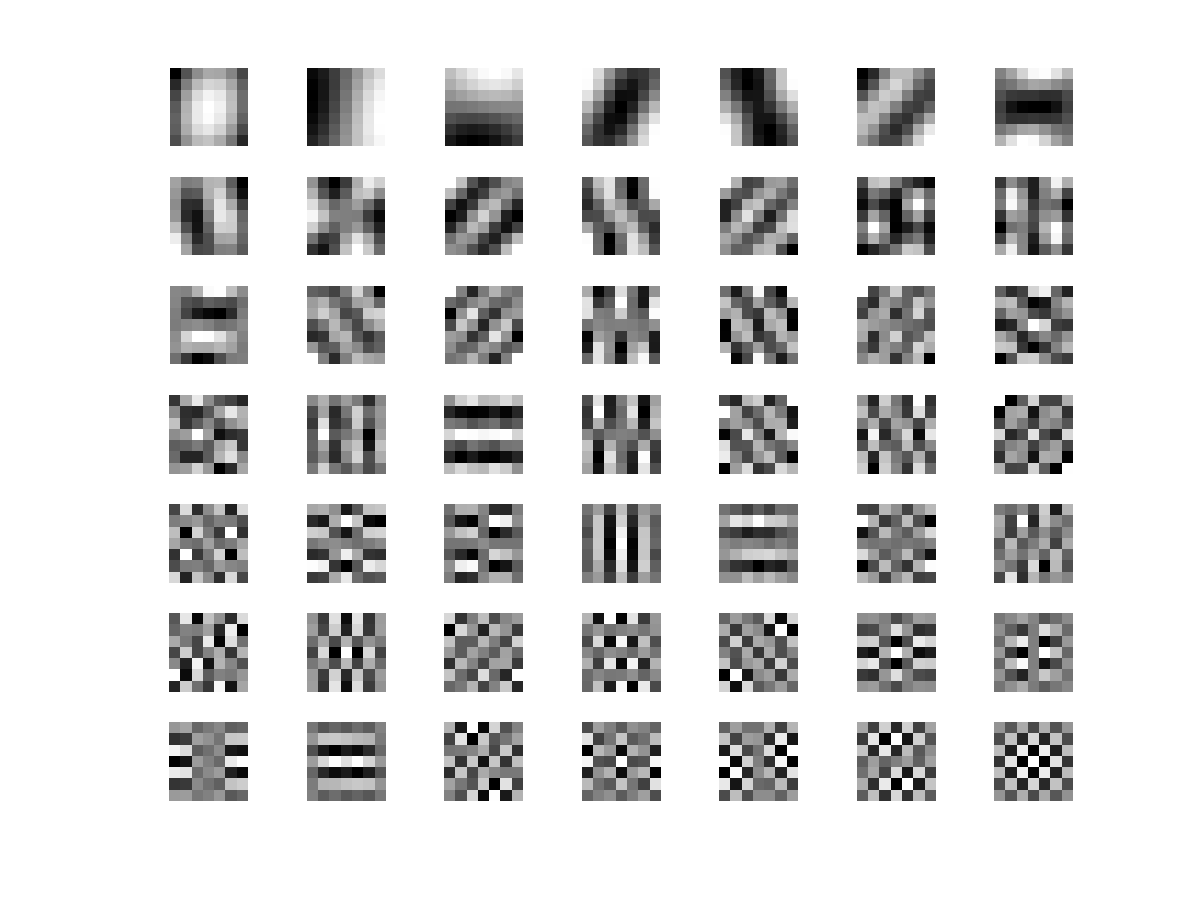
\includegraphics[width=\linewidth]{princomp_lena.png}
    \end{minipage}
      \caption{Left: the cosine basis; right: the principle components of zebra.jpg}
  \end{figure}      
 \end{frame}
 
 \begin{frame}
  \frametitle{Statistic : distribution of $\rand{C}_i$}
  \begin{itemize}
   \item The distribution of $\rand{C}_i$ is the empirical histogram of $\rand{C}_i$ over all the image
   \item We can also fit these distributions by a parametric distribution. (Gaussian, Laplacian ...)
  \end{itemize}

    \begin{figure}[h!]
    \centering
    \begin{minipage}{0.4\linewidth}
    \includegraphics<1-2>[width=\linewidth]{patch_1.png}
    \includegraphics<3-4>[width=\linewidth]{patch_2.png}
    \includegraphics<5-6>[width=\linewidth]{patch_3.png}
    \includegraphics<7-8>[width=\linewidth]{patch_4.png}
    \end{minipage}
    \begin{minipage}{0.4\linewidth}
    \includegraphics<1>[width=\linewidth]{h_1.png}
    \includegraphics<2>[width=\linewidth]{h_1_gau.png}
    \includegraphics<3>[width=\linewidth]{h_2.png}
    \includegraphics<4>[width=\linewidth]{h_2_gau.png}
    \includegraphics<5>[width=\linewidth]{h_3.png}
    \includegraphics<6>[width=\linewidth]{h_3_gau.png}
    \includegraphics<7>[width=\linewidth]{h_4.png}
    \includegraphics<8>[width=\linewidth]{h_4_gau.png}
    \end{minipage}
      \caption{Left: the cosine basis; right: the principle components of zebra.jpg}
  \end{figure}  
 \end{frame}

 
\begin{frame}
\frametitle{Statistic : distribution of $\rand{C}_i$}
      \begin{figure}[h!]
      \centering
      \begin{minipage}{0.8\linewidth}
      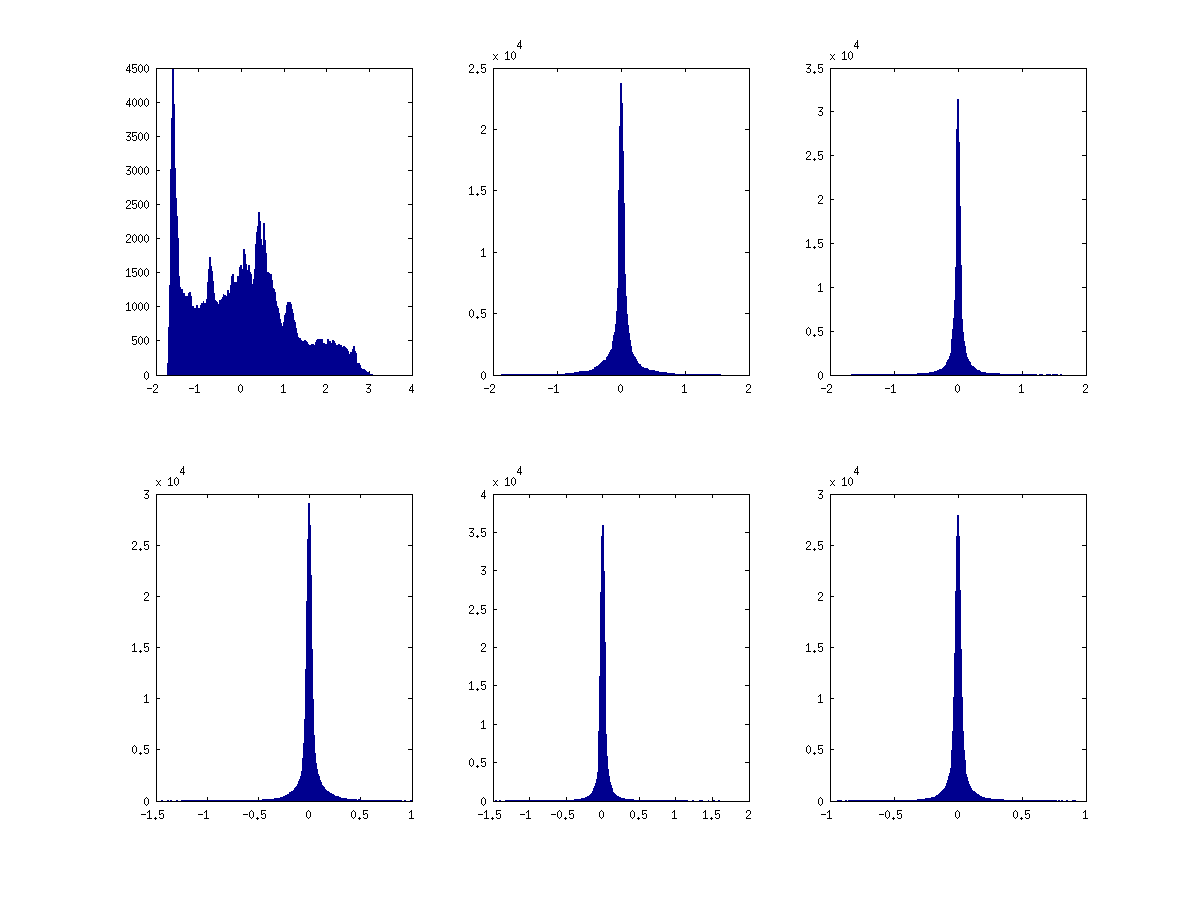
\includegraphics[width=\linewidth]{hist}
	
      \end{minipage}

	  \caption{Left: distribution of the first component; right: histogram of the image}
      
      \end{figure}      
\end{frame}
 
\begin{frame}
\frametitle{Statistic :}
      \begin{figure}[h!]
      \centering
      \begin{minipage}{0.8\linewidth}
      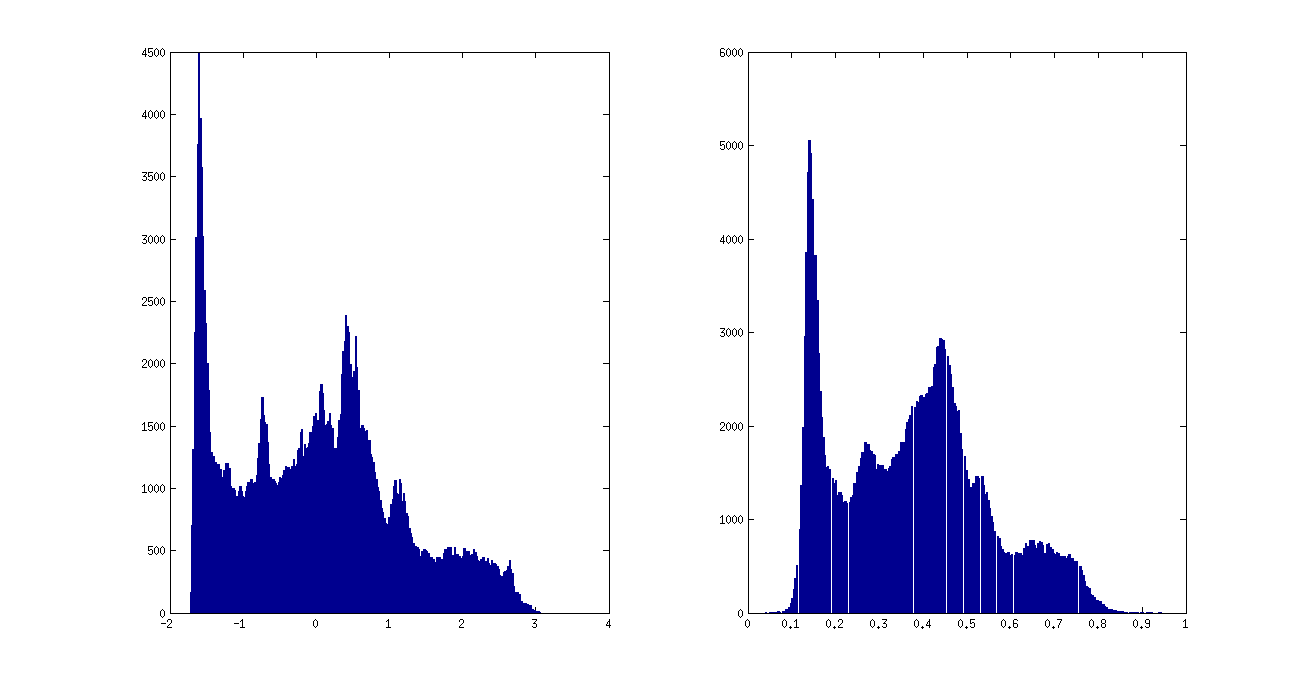
\includegraphics[width=\linewidth]{h_1vs_hist}
      \end{minipage}
	  \caption{Distribution of the firsts components}
      \end{figure}     
\end{frame}

 \section{Likelihood ration}
 
\begin{frame}
 \scriptsize
 {
 \begin{enumerate}


  \item A contrario method
  \item \textbf{Likelihood ratio}
  \item Likelihood ratio with learned prior
  \item Comparison
  
 \end{enumerate}

  %\frametitle{Table of contents}
  %\tableofcontents
  
 }
 \end{frame} 
 
 \begin{frame}
\frametitle{Likelihood method}
 \scriptsize
 {
 \begin{enumerate}
 \item Exhibit a statistical test to know if two patches are similar
 \item We assume each patch $\mathbf{x}$ is issued from a noise-free patch $\theta$ with some noise. E.g., if the noise is normal, $\mathbf(x) = \theta + \mathbf{n}$ where $n \sim \mathcal{N}(0,\sigma)$
 \item We consider and compare the null hypothesis $\mathcal{H}_0 : \theta_1=\theta2$ and the alternative hypothesis $\mathcal{H}_1 : \theta_1\neq\theta_2$
 \end{enumerate}
 }
\end{frame}
\begin{frame}
\frametitle{Likelihood ratio}
The Bayesian likelihood ratio considers a known prior
\begin{align*}
L_B(\mathbf{x_1},\mathbf{x_2})&=\frac{p(\mathbf{x_1},\mathbf{x_2};\mathcal{H}_0)}{p(\mathbf{x_1},\mathbf{x_2};\mathcal{H}_1)}\\
&=\frac{\int p(\mathbf{x_1}|\mathbf{\theta_{12}}=t)p(\mathbf{x_2}|\mathbf{\theta_{12}}=t)p(\mathbf{\theta_{12}}=\mathbf{t})\mathrm{d}\mathbf{t}}{\prod_{i=1,2}\int p(\mathbf{x_i}|\mathbf{\theta_i})\mathbf{t_i})p(\mathbf{\theta_i}=\mathbf{t_i})\mathrm{d}\mathbf{t_i}}
\end{align*}
The prior can be non-informative, such as a Jeffreys prior.
\end{frame}

\begin{frame}
\frametitle{Likelihood ratio}
The generalized likelihood ratio uses the maximum likelihood estimates for the noise-free patches.
\[
L_G(\mathbf{x_1},\mathbf{x_2})=\frac{\sup_\mathbf{t}p(\mathbf{x_1},\mathbf{x_2};\theta_{12}=\mathbf{t},\mathcal{H}_0)}
{\sup_{t_1,t_2}p(x_1,x_2 \arrowvert \theta_1=t_1,\; \theta_2=t_2 , \mathcal{H}_1)}
\]
This comes down to using euclidian distance when the prior is non-informative.
\end{frame}
 
 \section{Likelihood ration with learned prior}
 \begin{frame}
 \scriptsize
 {
 \begin{enumerate}


  \item A contrario method
  \item Likelihood ratio
  \item \textbf{Likelihood ratio with learned prior}
  \begin{enumerate}
   \item motivation
   \item approach
  \end{enumerate}

  \item Comparison
  
 \end{enumerate}

  %\frametitle{Table of contents}
  %\tableofcontents
  
 }
 \end{frame} 
 
 \begin{frame}
  \frametitle{Motivation}
   \begin{itemize}
    \item{\textbf{Motivation}} Previous approach : image patches are considered as a white noise (c.f. section Comparison).
    \item{\textbf{Objective}} Introduce the prior information proposed by the a-constrario method, into the likelihood ratio.
   \end{itemize}
   \insertTwoF{lena.jpg}{wn}{}{0.4}
 \end{frame}
 
 \begin{frame}
  \frametitle{Approach : likelihood ratio}
  \begin{itemize}
   \item likelihood ratio :
   \begin{equation}
    \mathcal{L}=\frac{P(x_1,x_2 \arrowvert \mathcal{H}_0)}{P(x_1,x_2 \arrowvert \mathcal{H}_1)}
   \end{equation}
   \item we use the prior information $p(\theta_{12}) d\theta_{12}=\prod_i h_i(c_i)dc_i$ to compute this ratio
   \begin{equation}
   \begin{split}
       P(x_1,x_2 \arrowvert \mathcal{H}_0)&=\int P(x_1 \arrowvert \theta_{12}) P(x_2 \arrowvert \theta_{12}) p(\theta_{12}) d\theta_{12}\\
       &=\int P(x_1 \arrowvert \theta_{12}) P(x_2 \arrowvert \theta_{12}) \prod_i h_i(c_i)dc_i\\
   \end{split}
   \end{equation}
   \item for gaussian noise : $P(x \arrowvert \theta_{12})\propto \exp (- 1/\sigma^2  \lVert x-\theta_{12} \rVert^2) $
   \item orthogonal component $ +$ univariate gaussian noise $\longrightarrow$ separable integral! 
  \end{itemize}
 \end{frame}
 
 \begin{frame}
  \frametitle{Approach : maximum likelihood ratio}

   \begin{equation}
   \begin{split}
       P(x_1 \arrowvert \mathcal{H}_1)&=\int P(x_1 \arrowvert \theta_{1})  p(\theta_{1}) d\theta_{1}\\
       &=\int \exp (- 1/\sigma^2  \lVert x_1-\theta_{1} \rVert^2)  \prod_i h_i(c_i)dc_i\\
       &=\int \exp (- 1/\sigma^2  \lVert \sum _i (cx_i -c_{i})\mat B_i \rVert^2)  \prod_i h_i(c_i)dc_i\\
       &=\prod_i \int \exp (- 1/\sigma^2  \lVert (cx_i -c_{i}) \rVert^2)   h_i(c_i)dc_i\\
   \end{split}
   \end{equation}
   \insertF{corr}{Distribution of $\rand{C}_i$}{0.3}
 \end{frame}
 
  \begin{frame}
   \frametitle{Approach : generalized likelihood ratio}
   \begin{itemize}
    \item Maximum a posteriori (Gaussian approximation for the prior) 
   \begin{equation}
   \begin{split}
       \mathcal{Q}&=\sup_{\theta_{12}} P(x_1 \arrowvert \theta_{12}) P(x_2 \arrowvert \theta_{12}) p(\theta_{12})\\
       &=\prod_i  \sup_{c_i}  \exp (- 1/\sigma^2  \lVert (cx_i -c_{i}) \rVert^2- 1/\sigma^2  \lVert (cx_i -c_{i}) \rVert^2 \\
       &- 1/\sigma_i^2  \lVert (c_{i}-\mu_i) ) 
   \end{split}
   \end{equation}
   \item $\hat c_i=(a (x_1+x_2)+\mu_i)/(1+2a)$ where $a=(\sigma_i /\sigma)^2$
   \insertF{corr}{Distribution of $\rand{C}_i$}{0.3}
   \end{itemize}

 \end{frame}
 
  \begin{frame}
  \frametitle{Approach : generalized likelihood ratio}
   \insertTwoF{curve}{corr}{ In blue, The similarity as a function of $\sigma_i$, the standard deviation of $\rand{C}_i$; in red, the euclidian distance }{0.45}
 \end{frame}
 
 
 \section{Comparison}
  \begin{frame}
 \scriptsize
 {
 \begin{enumerate}


  \item A contrario method
  \item Likelihood ratio
  \item {Likelihood ratio with learned prior}
  \item \textbf{Comparison}
  
 \end{enumerate}

  %\frametitle{Table of contents}
  %\tableofcontents
  
 }
 \end{frame}

\begin{frame}
\frametitle{Results for different methods}
\begin{figure}
\centering
\begin{minipage}{0.3\linewidth}
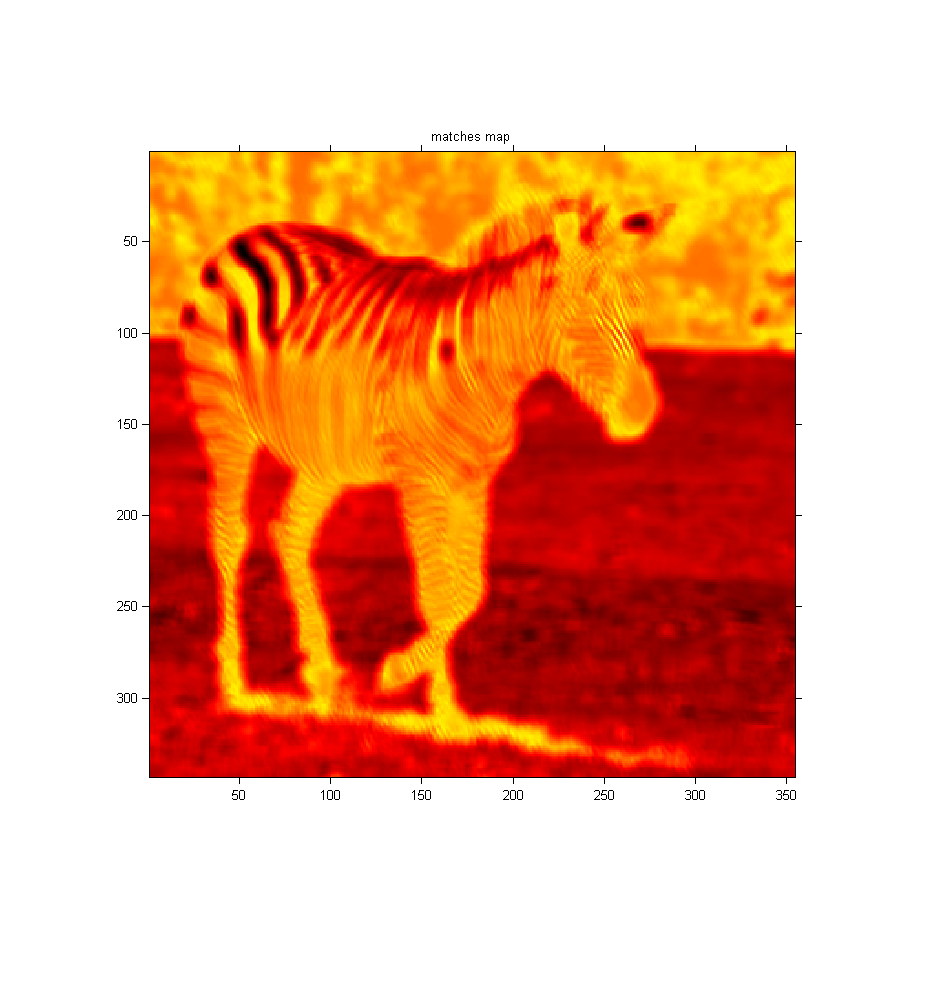
\includegraphics[width=1.3\linewidth]{zebra_heatmap_euclidian.png}
\end{minipage}
\begin{minipage}{0.3\linewidth}
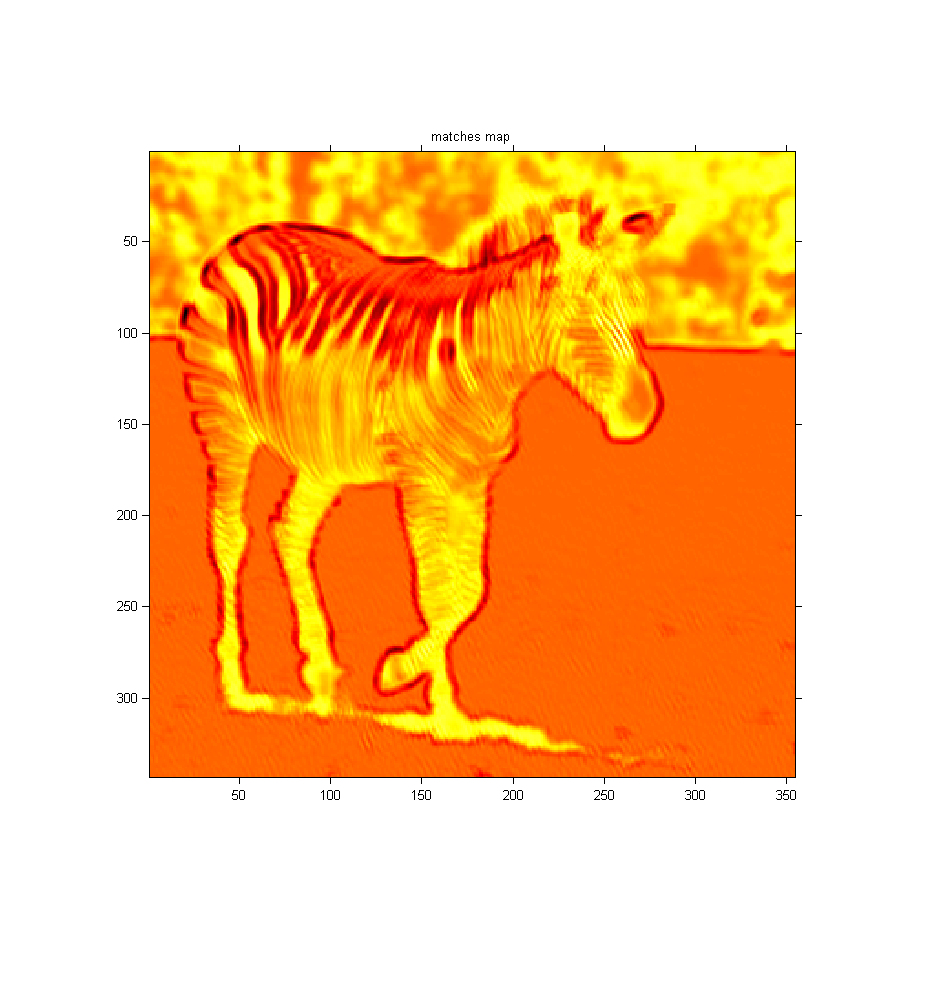
\includegraphics[width=1.3\linewidth]{zebra_heatmap_similarity.png}
\end{minipage}
\begin{minipage}{0.3\linewidth}
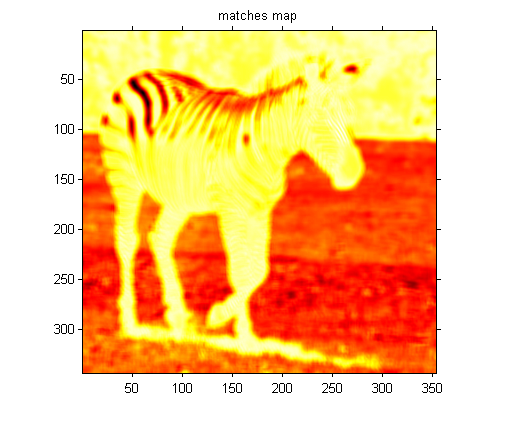
\includegraphics[width=1.3\linewidth]{zebra_heatmap_approx.png}
\end{minipage}
\end{figure}
\end{frame}

\begin{frame}
\frametitle{Results for different methods}
\begin{figure}
\centering
\begin{minipage}{0.3\linewidth}
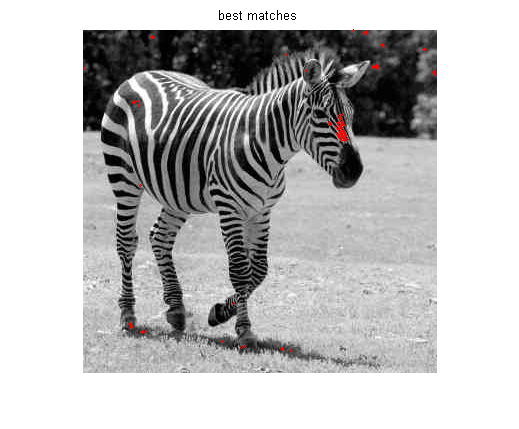
\includegraphics[width=1.3\linewidth]{zebra_best_matches_euclidian.png}
\end{minipage}
\begin{minipage}{0.3\linewidth}
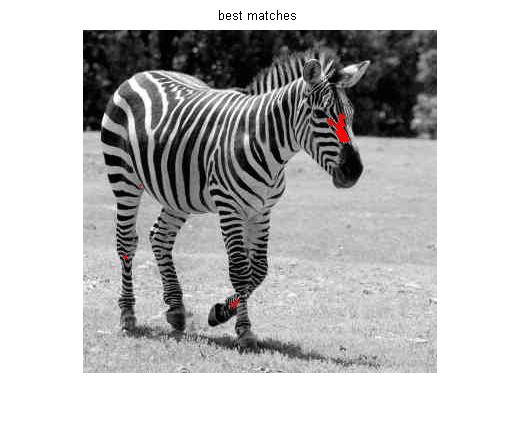
\includegraphics[width=1.3\linewidth]{zebra_best_matches_similarity.png}
\end{minipage}
\begin{minipage}{0.3\linewidth}
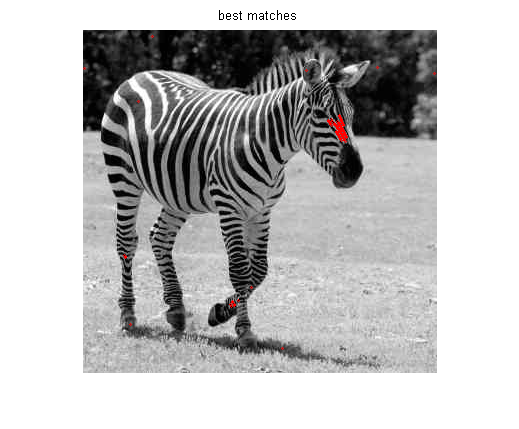
\includegraphics[width=1.3\linewidth]{zebra_best_matches_approx.png}
\end{minipage}
\end{figure}
\end{frame}

  
  \begin{frame}
  \frametitle{Performance PFA versus PTD}
   \insertTwoF{zebra.jpg}{perf_zebra_max}{ method max }{0.45}
 \end{frame}
 
   \begin{frame}
  \frametitle{Performance PFA versus PTD}
   \insertTwoF{lena.jpg}{perf_texture_max}{ method max  }{0.45}
 \end{frame}
 
  
   \begin{frame}
  \frametitle{Performance PFA versus PTD}
   \insertTwoF{wn}{perf_wn_max}{ method max  }{0.45}
 \end{frame}
 
  \begin{frame}
  \frametitle{Performance PFA versus PTD}
   \insertTwoF{zebra.jpg}{perf_zebra_int}{ method int }{0.45}
  \end{frame}
 
  \begin{frame}
  \frametitle{Performance PFA versus PTD}
   \insertF{perf_zebra_max}{ method max }{0.8}
 \end{frame}
   \begin{frame}
  \frametitle{Performance PFA versus PTD}
   \insertF{perf_zebra_int}{ method int}{0.8}
 \end{frame}
 
% \begin{frame}
%  \frametitle{Conclusion}
%  \begin{itemize}
%   \item Planar mirror calibration : [Sturm & Bonfort 2006] [R. Kumar \textit{et al.} 2008], [Rodrigues \textit{et al.} 2010] 
%   \begin{itemize}
%    \item Simple acquisition device and fast feature detection (could be used on random planar pattern)
%    \item efficient algorithm and fast resolution
%    \item minimum 3 views are required
%    \item less precise in translation estimation  
%   \end{itemize}
%   \item Spherical mirror calibration : [Agrawal 2013]
%  \begin{itemize}
%    \item 1 view calibration without ambiguity
%    \item higher precision
%    \item more complex device
%    \item sophistic feature detection method
%   \end{itemize}
%  \end{itemize}
% 
% \end{frame}

  \begin{frame}
   {\Huge
     \vspace {0.15\textwidth}
     \begin{columns}
       \begin{column}{0.3\textwidth}
       \end{column}
       \begin{column}{0.3\textwidth}
        \text{Thank you!}
       \end{column}
       \begin{column}{0.3\textwidth}
       \end{column}
     \end{columns}
   }
   \vspace {0.025\textwidth}
   \begin{center}
   {\huge Q\&A}
   \end{center}
 \end{frame}
  
\end{document}